\documentclass{beamer}
\usepackage{graphicx}
\usepackage{amsmath}
\begin{document}
\title{Public Key Infrastructure}
\subtitle{Introduction to cryptography}
\author{Bruce Ricard, VMware}
\date{April 30th, 2020}

\frame{\titlepage}

\frame{\
  \frametitle{Agenda}
  \tableofcontents
}

\section{Prerequisites}
\subsection{Cryptography}
\frame{
  \frametitle{Cryptography}
  \framesubtitle{A little history}

  Caesar cipher
  \pause
  \begin{figure}
  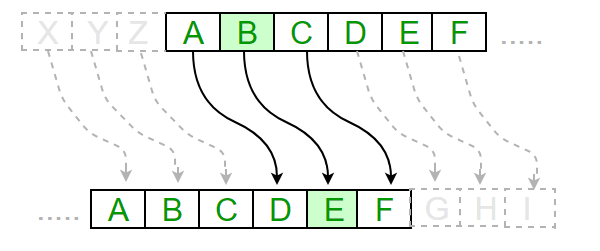
\includegraphics[scale=0.3]{images/caesar_cipher.png}
  \end{figure}

  Example: $``I LOVE CRYPTOGRAPHY'' \rightarrow
  ``L ORYH FUBSWRJUDSKB''$

  \pause

  \vspace{\baselineskip}
  Symmetric(-Key) Cryptography
}

\frame{
  \frametitle{Cryptography}
  \framesubtitle{Vocabulary}

  Symmetric Cryptography diagram:

  plain text $\xrightarrow[key]{encryption}$
  cipher $\xrightarrow[key]{decryption}$ plain text

  TODO: add examples here
}

\frame{
  \frametitle{Cryptography}
  \framesubtitle{Issues with symmetric cryptography}

  Sharing key with other parties
  Different key for every party

  --> leads to public key cryptography
}

\frame{
  \frametitle{Cryptography}
  \framesubtitle{Public key cryptography}

  One way functions
}

\frame{
  \frametitle{Cryptography}
  \framesubtitle{Public key cryptography}

  RSA (Rivest–Shamir–Adleman 1977)

  TODO: quick example on some fairly small finite field
}

\frame{
  \frametitle{Cryptography}
  \framesubtitle{Issues with public key cryptography}

  Slow, can only encrypt little data
  (kinda by design -- one-way functions)

  Anybody can encrypt data: no more sender validation

  --> leads to signatures
}



\frame{
  \frametitle{Cryptography}
  \framesubtitle{Encrypting / Decrypting}
  \begin{itemize}
  \item Symetric (AES)
  \item Asymetric or public key (RSA)
  \end{itemize}
  \pause
  Symetric: need to exchange keys, need different key for each person you want to exchange with \\
  Asymetric: can only encrypt small amounts of data, slower/heavier algorithm usually
}

\frame{
  \frametitle{Cryptography}
  \framesubtitle{Signing / Validating}

  Use asymetric cryptography to sign: ``encrypt'' with private key.
}

\frame{
  \frametitle{Cryptography}

  Questions?
}


\section{Communicating safely using cryptography}
\frame{
  \frametitle{Using cryptography to communicate safely}

  \begin{itemize}
  \item Encrypt data so that it can only be read by entity with decoding key
  \item Making sure that the right entity has the decoding key
  \end{itemize}

  \pause
  \begin{itemize}
  \item Encrypt AES key with RSA
  \item Sign RSA public keys / owner by trusted party \pause : certificates
  \end{itemize}
}

\subsection{Certificates}
\frame{
  \frametitle{Certificates}
  \framesubtitle{identity}

  e-ID for software \pause

  \begin{itemize}
  \item CA
  \item RA
  \item x509 \pause
    \begin{itemize}
    \item Name / url
    \item public key
    \item trusted signature
    \end{itemize}
  \end{itemize}
}

\frame{
  \frametitle{Certificates}

  Questions?
}


\subsection{SSL / TLS}
\frame{
  \frametitle{SSL / TLS}
  \framesubtitle{TLS - Transport Layer Security}
  \begin{itemize}
  \item Cryptographic protocol for safe communication over computer network
    \pause
  \item Previously: SSL - Secure Sockets Layer (1994)
    \pause
  \item TLS 1.0 (1999)
  \item Now TLS 1.3 (2018)
  \end{itemize}
}


\frame{
  \frametitle{SSL / TLS}
  \framesubtitle{TLS handshake (simplified)}

  \pause
  \begin{enumerate}
  \item Client makes $https$ call to server: initiates TLS handshake
  \item Server sends its $x509$ certificate
  \item Client validates certificate signature against CA
  \item Client validates certificate hostname and gets public key $p$
  \item Client generates random string to be symetric private key $k$
  \item Client encrypt $k$ with server's public key $p$, and sends it to the server
  \item Server decrypts encoded key with its private key
  \end{enumerate}

  \pause
  End of handshake:
  \begin{itemize}
  \item client validated identity of server
  \item both parties have secure secret key for encrypted private communication
  \end{itemize}

  \pause
  Server and client will now communicate by encoding and decoding any data sent
  over the wire with their private key, using a symetric algorithm like AES.
}

\frame{
  \frametitle{How does TLS work?}
  \framesubtitle{Why is it secure?}

  \begin{itemize}
  \item encrypts data
  \item makes sure the right entity can decrypt
  \end{itemize}
}

\frame{
  \frametitle{TLS}

  Questions?
}

\frame{
  \frametitle{TLS}
  \framesubtitle{What is --skip-ssl-validation?}

  Or in the browser ``This page in not secure...''
  \pause

  Not encrypting data? \pause Yes it is.
  Not validating identity.
}

\frame{
  \frametitle{mTLS}
  \framesubtitle{mutual TLS}

  \begin{itemize}
  \item With TLS, client validates identity of server. Client doesn't authenticate.
  \item Most websites use username/password for client authentication.
  \item mTLS can be done with username/password: we'll look at certificate based mTLS
  \end{itemize}

  \pause
  Not MTLS
}

\frame{
  \frametitle{mTLS}
  \framesubtitle{mutual TLS}

  \begin{enumerate}
  \item server sends its certificate to client
  \item client validates certificate signature and hostname
  \item client sends its certificate to server
  \item server validates certificate signature
  \item server generates random key to use as private symmetric key and sends
    to client
  \end{enumerate}

  \pause

  Both entities validated that the other party is trustworthy
}

\frame{
  \frametitle{mTLS}
  \framesubtitle{TLS termination}

  \begin{itemize}
  \item TLS termination proxy
  \item TLS forward proxy
  \end{itemize}
  \pause
  CF does mostly TLS forward proxy, calls it TLS termination proxy
}


\section{PKI}
\subsection{What is a public key infrastructure?}
\frame{
  \frametitle{PKI}

  A PKI consists of:
  \begin{itemize}
  \item A certificate authority (CA)
  \item A registration authority (RA)
  \item A central directory (for key storage)
  \item A certificate management system (e.g. who can access the stored keys)
  \item A certificate policy (stating the PKI's requirements concerning its procedures.
    Its purpose is to allow outsiders to analyze the PKI's trustworthiness.)
  \end{itemize}
}

\section{Extras}

\frame{
  \frametitle{Safe key exchange}
  \framesubtitle{Diffie Helmann}

  \begin{itemize}
  \item Issue with exchanging private keys with symmetric algorithm
    if private key gets lost
  \item Diffie Helmann algorithm
  \end{itemize}
}
\end{document}
